%%%%%%%%%%%%%%%%%%%%%%%%%%%%%%%%%%%%%%%%%
% Masters/Doctoral Thesis 
% LaTeX Template
% Version 1.43 (17/5/14)
%
% This template has been downloaded from:
% http://www.LaTeXTemplates.com
%
% Original authors:
% Steven Gunn 
% http://users.ecs.soton.ac.uk/srg/softwaretools/document/templates/
% and
% Sunil Patel
% http://www.sunilpatel.co.uk/thesis-template/
%
% License:
% CC BY-NC-SA 3.0 (http://creativecommons.org/licenses/by-nc-sa/3.0/)
%
% Note:
% Make sure to edit document variables in the Thesis.cls file
%
%%%%%%%%%%%%%%%%%%%%%%%%%%%%%%%%%%%%%%%%%

%% thesis template used by Peter Krieg, Physics Major at Bates college for senior thesis

%----------------------------------------------------------------------------------------
%	PACKAGES AND OTHER DOCUMENT CONFIGURATIONS
%----------------------------------------------------------------------------------------

\documentclass[11pt, oneside]{Thesis} % The default font size and one-sided printing (no margin offsets)

\graphicspath{{Pictures/}} % Specifies the directory where pictures are stored

\usepackage[square, numbers, comma, sort&compress]{natbib} % Use the natbib reference package - read up on this to edit the reference style; if you want text (e.g. Smith et al., 2012) for the in-text references (instead of numbers), remove 'numbers' 
\usepackage{listings}
\usepackage{color}
\usepackage{xcolor}
\usepackage{textcomp}   %Iuse this for the degree symbol
\usepackage{amsmath}  % use for making bigger math symbols
\usepackage{relsize}  % use for making bigger math symbols



\usepackage{caption}
\DeclareCaptionFont{black}{\color{black}}
\DeclareCaptionFormat{listing}{\parbox{\textwidth}{#1#2#3}}
\captionsetup[lstlisting]{format=listing,labelfont=black,textfont=black}



\hypersetup{urlcolor=black, colorlinks=false} % Colors hyperlinks in blue - change to black if annoying

\title{\ttitle} % Defines the thesis title - don't touch this

\begin{document}

\frontmatter % Use roman page numbering style (i, ii, iii, iv...) for the pre-content pages

\setstretch{1.3} % Line spacing of 1.3

% Define the page headers using the FancyHdr package and set up for one-sided printing
\fancyhead{} % Clears all page headers and footers
\rhead{\thepage} % Sets the right side header to show the page number
\lhead{} % Clears the left side page header

\pagestyle{fancy} % Finally, use the "fancy" page style to implement the FancyHdr headers

\newcommand{\HRule}{\rule{\linewidth}{0.5mm}} % New command to make the lines in the title page

% PDF meta-data
\hypersetup{pdftitle={\ttitle}}
\hypersetup{pdfsubject=\subjectname}
\hypersetup{pdfauthor=\authornames}
\hypersetup{pdfkeywords=\keywordnames}

%----------------------------------------------------------------------------------------
%	TITLE PAGE
%----------------------------------------------------------------------------------------

\begin{titlepage}
\begin{center}

\textsc{\LARGE \univname}\\[1.5cm] % University name
\textsc{\Large Senior Thesis}\\[0.5cm] % Thesis type

\HRule \\[0.4cm] % Horizontal line
{\huge \bfseries \ttitle}\\[0.4cm] % Thesis title
\HRule \\[1.5cm] % Horizontal line
 
\begin{minipage}{0.4\textwidth}
\begin{flushleft} \large
\emph{Author:}\\
\href{http://www.peterkrieg.com/thesis}{\authornames} % Author name - remove the \href bracket to remove the link
\end{flushleft}
\end{minipage}
\begin{minipage}{0.4\textwidth}
\begin{flushright} \large
\emph{Advisor:} \\
\supname % Supervisor name - remove the \href bracket to remove the link  
\end{flushright}
\end{minipage}\\[3cm]
 
\large \textit{Presented to The Department of Physics, Bates College\\ In Partial Fulfillment of the Requirements for the \\ Degree of Bachelor of Science}\\[0.3cm] % University requirement text

\

 \large Lewiston, Maine 
 \

{\large December 1st, 2014}\\[2cm] % Date

\includegraphics[width=4cm, height=4cm]{logotransparent.png} % University/department logo - uncomment to place it
 
\vfill
\end{center}

\end{titlepage}

%----------------------------------------------------------------------------------------
%	DECLARATION PAGE
%	Your institution may give you a different text to place here
%----------------------------------------------------------------------------------------

\Declaration{

\addtocontents{toc}{\vspace{1em}} % Add a gap in the Contents, for aesthetics

I, \authornames, declare that this thesis titled, `\ttitle' and the work presented in it are my own. I confirm that:

\begin{itemize} 
\item[\tiny{$\blacksquare$}] This work was done wholly or mainly while in candidature for a research degree at this College.
\item[\tiny{$\blacksquare$}] Where any part of this thesis has previously been submitted for a degree or any other qualification at this University or any other institution, this has been clearly stated.
\item[\tiny{$\blacksquare$}] Where I have consulted the published work of others, this is always clearly attributed.
\item[\tiny{$\blacksquare$}] Where I have quoted from the work of others, the source is always given. With the exception of such quotations, this thesis is entirely my own work.
\item[\tiny{$\blacksquare$}] I have acknowledged all main sources of help.
\item[\tiny{$\blacksquare$}] Where the thesis is based on work done by myself jointly with others, I have made clear exactly what was done by others and what I have contributed myself.\\
\end{itemize}
 
Signed:\\
\rule[1em]{25em}{0.5pt} % This prints a line for the signature
 
Date:\\
\rule[1em]{25em}{0.5pt} % This prints a line to write the date
}

\clearpage % Start a new page
\clearpage

%----------------------------------------------------------------------------------------
%	QUOTATION PAGE
%----------------------------------------------------------------------------------------

% \pagestyle{empty} % No headers or footers for the following pages

% \null\vfill % Add some space to move the quote down the page a bit

% \textit{``Thanks to my solid academic training, today I can write hundreds of words on virtually any topic without possessing a shred of information, which is how I got a good job in journalism."}

% \begin{flushright}
% Dave Barry
% \end{flushright}

% \vfill\vfill\vfill\vfill\vfill\vfill\null % Add some space at the bottom to position the quote just right

% \clearpage % Start a new page

%----------------------------------------------------------------------------------------
%	ABSTRACT PAGE
%----------------------------------------------------------------------------------------

\addtotoc{Abstract} % Add the "Abstract" page entry to the Contents

\abstract{\addtocontents{toc}{\vspace{1em}} % Add a gap in the Contents, for aesthetics


This thesis outlines the programming necessary to simulate various mechanical phenomena in physics.  The simulations are programmed using JavaScript, and viewable in a web browser through the HTML5 canvas API.  Please visit http://peterkrieg.com/thesis to view all of the simulations.  Each chapter investigates a different topic of mechanics, with simulations for each.  The first chaper investigates basic kinematics and aerodynamic drag through balls bouncing.  The second chapter presents simulations for orbiting bodies, and investigates Kepler's 2nd law of planetary motion.  The third chapter examines angular momentum, torque, and Newton's Second Law for rotation.  





}

\clearpage % Start a new page

%----------------------------------------------------------------------------------------
%	ACKNOWLEDGEMENTS
%----------------------------------------------------------------------------------------

\setstretch{2} % Reset the line-spacing to 2 for acknowledgements text (if it has changed)

\acknowledgements{\addtocontents{toc}{\vspace{1em}} % Add a gap in the Contents, for aesthetics

\vspace{1cm}
First and foremost, I would like to thank my advisor, Gene Clough.  Gene, thank you for your guidance along the way: you helped me to formulate my ideas and you encouraged me throughout the semester.  I appreciate your patience and dedication to working with me--I have always enjoyed discussing problems with you.  I feel relieved walking into your office knowing that you will have a book pertaining to any problem I'm having.

I would also like to thank Professor Hong Lin, who met with me multiple different times to discuss my thesis.  Thank you, Professor Lin, for thoroughly explaining concepts with me and for letting me borrow some of your books.  Additionally, thank you to Professor Mark Semon, for showing me past examples of theses, and outlining the formatting requirements for Bates.  Thank you to the Ladd Library staff for helping me with research. 

I would like to acknowledge Steven Gunn, who wrote the original LaTeX template that this thesis uses.  All of the formatting and aesthetics of my thesis are thanks to his hard work, I only inputted my own content.

I would like to acknowledge Dev Ramtal and Adrian Dobre for their helpful book, ``Physics for JavaScript Games, Animation, and Simulations''.  While the code presented in this thesis was completely written by me, I used external libraries of code at times to speed up the development process.  This code is cited when necessary throughout the thesis, and was approved by my advisor Gene.   

Thank you to my parents for encouraging me throughout the whole process, and for at least trying to understand what I was doing for my thesis.  I would also like to thank my friends and classmates who supported my work.

Lastly I would like to thank the variety of online resources that helped me with coding challenges along the way.  Stackoverflow was particularly useful with JavaScript and LaTeX problems I encountered.      


}
\clearpage % Start a new page

%----------------------------------------------------------------------------------------
%	LIST OF CONTENTS/FIGURES/TABLES PAGES
%----------------------------------------------------------------------------------------

\pagestyle{fancy} % The page style headers have been "empty" all this time, now use the "fancy" headers as defined before to bring them back

\lhead{\emph{Contents}} % Set the left side page header to "Contents"
\tableofcontents % Write out the Table of Contents

% \lhead{\emph{List of Figures}} % Set the left side page header to "List of Figures"
% \listoffigures % Write out the List of Figures

% \lhead{\emph{List of Tables}} % Set the left side page header to "List of Tables"
% \listoftables % Write out the List of Tables

%----------------------------------------------------------------------------------------
%	ABBREVIATIONS
%----------------------------------------------------------------------------------------

% \clearpage % Start a new page

% \addtocontents{toc}{\vspace{1em}}
% \setstretch{1.5} % Set the line spacing to 1.5, this makes the following tables easier to read

% \lhead{\emph{Abbreviations}} % Set the left side page header to "Abbreviations"
% \listofsymbols{ll} % Include a list of Abbreviations (a table of two columns)
% {

% \textbf{HTML} &   HyperText Markup Language \\
% \textbf{JS} & JavaScript \\
% \textbf{API} &  Application Programming Interface
% }

%----------------------------------------------------------------------------------------
%	PHYSICAL CONSTANTS/OTHER DEFINITIONS
%----------------------------------------------------------------------------------------

% \clearpage % Start a new page

% \lhead{\emph{Physical Constants}} % Set the left side page header to "Physical Constants"

% \listofconstants{lrcl} % Include a list of Physical Constants (a four column table)
% {
% Speed of Light & $c$ & $=$ & $2.997\ 924\ 58\times10^{8}\ \mbox{ms}^{-\mbox{s}}$ (exact)\\
% % Constant Name & Symbol & = & Constant Value (with units) \\
% }

%----------------------------------------------------------------------------------------
%	SYMBOLS
%----------------------------------------------------------------------------------------

% \clearpage % Start a new page

% \lhead{\emph{Symbols}} % Set the left side page header to "Symbols"

% \listofnomenclature{lll} % Include a list of Symbols (a three column table)
% {
% $a$ & distance & m \\
% $P$ & power & W (Js$^{-1}$) \\
% % Symbol & Name & Unit \\

% & & \\ % Gap to separate the Roman symbols from the Greek

% $\omega$ & angular frequency & rads$^{-1}$ \\
% % Symbol & Name & Unit \\
% }

%----------------------------------------------------------------------------------------
%	DEDICATION
%----------------------------------------------------------------------------------------

% \setstretch{1.3} % Return the line spacing back to 1.3

% \pagestyle{empty} % Page style needs to be empty for this page

% \dedicatory{Dedicated to my parents} % Dedication text

% \addtocontents{toc}{\vspace{2em}} % Add a gap in the Contents, for aesthetics

%----------------------------------------------------------------------------------------
%	THESIS CONTENT - CHAPTERS
%----------------------------------------------------------------------------------------

\mainmatter % Begin numeric (1,2,3...) page numbering

\pagestyle{fancy} % Return the page headers back to the "fancy" style

% Include the chapters of the thesis as separate files from the Chapters folder
% Uncomment the lines as you write the chapters


\addtocontents{toc}{\hspace{-2em}}  \addtocontents{toc}{\textbf{Introduction}} %This adds an introduction item to table of contents, just for aesthetic look






\setstretch{2}


% Introduction

\chapter*{Introduction}
\label{intro} % For referencing the chapter elsewhere, use \ref{Chapter1} 

\lhead{Introduction \emph{ Presenting the basics of a physics simulation}} % This is for the header on each page - perhaps a shortened title

%----------------------------------------------------------------------------------------

\section{What is a Physics Simulation?}

\hspace{.5cm} The purpose of this thesis is to present a series of physics simulations, each modeling a specific problem of physics as realistically as possible.  These simulations differ from \textit{animations}, which are predictable representations that always display the same visual.  Animations are analagous to a movie script: they always end in the same way.  Simulations, on the other hand, need to adapt to variable conditions, and may be based partly on random processes.  This brings up the topic of \textit{dynamic} vs. \textit{static} animation.  Most of the physics simulations in this thesis will be dyamic because they present a unique viewing each time they are run, and can also involve user input which influences the outcome of the simulation.

Any simulation requires creating the illusion of motion.  Almost every form of projected motion media uses frames to accomplish this.  Researchers have shown that to make a simulation look realistic, it must be presented at a rate of around 60-100 frames per second.\textsuperscript{\cite{jsbook}}  Anything slower and the human eye will detect the ``choppiness'' of the simulation.  People can't detect anything much faster than 100 frames per second, so there is no need to project media faster than that, with the exception of slow-motion videography.  




%----------------------------------------------------------------------------------------


\section{Methods of Producing a Simulation}

The physics simulations in this thesis differ greatly from common animations.  Movies and cartoons, for example, operate by displaying a series of images similar to one another, and displaying them as many frames per second to create the illusion of motion.  My simulations, on the other hand, function by providing the \textit{information} for each frame, and then providing the data for \textit{how} the animation can be created.  These instructions are passed onto the HTML5 canvas API, which creates the visual which can be seen in the web browser.\textsuperscript{\cite{basichtml5}}  Because physics simulations contain instructions instead of a series of images, the files of code take up far less space than a movie file would, for example.  This is one primary advantage of coded simulations.  Every simulation follows a similar set of steps, which can be simplified below: 

\begin{figure}[h] 
	\centering
		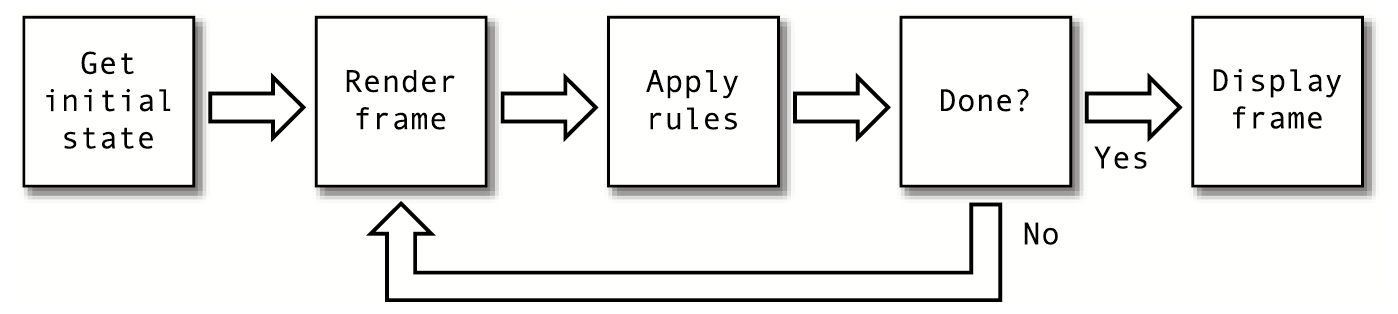
\includegraphics[width=15cm]{Figures/frames.png}

	\caption{The frames of a general simulation}
	\label{fig:frames}
\end{figure}


The canvas API gets the initial state of the simulation, which could the position of a ball, for example.  Then, the frame is \textit{rendered} by applying rules to the canvas element, and changing the initial state of the simulation.  Once the rules have been applied, and all conditions are satisfied, the frame is rendered, and then displayed on the canvas element, to be seen in the web browser.\textsuperscript{\cite{basichtml5}}  The canvas is embedded into a web page with the \textless canvas\textgreater tag, like any other HTML tag.  The positioning of objects in the canvas element is specified with a coordinate system, which uses pixels as its unit.  Figure \ref{fig:canvas} shows the orientation of the canvas, which differs from the traditional cartesian coordinate system.

\begin{figure}[h] 
	\centering
		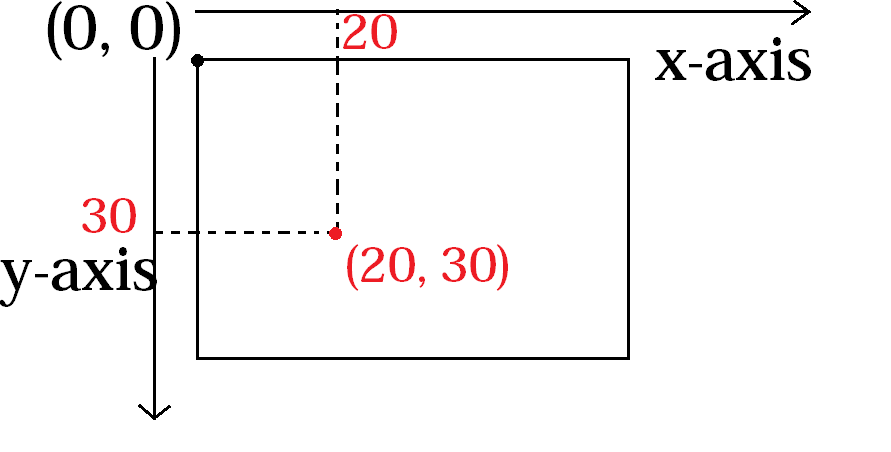
\includegraphics[width=8cm]{Figures/canvas.png}

	\caption{The canvas coordinate system.  The canvas is displayed on the screen as a white rectangle by default.  A sample point of (20,30) is shown for clarification.}
	\label{fig:canvas}
\end{figure}



To produce any realistic simulation, the steps in figure \ref{fig:frames} must be repeated multiple times per second.  In fact, these steps must be repeated 60 times per second to achieve the desired 60 frames per second outlined in the previous section.  Luckily, the canvas API is capable of running the instructions very quickly to make this simulation possible.  





%----------------------------------------------------------------------------------------





\subsection{The Code}

To program the simulations in this thesis, I chose to write the code in JavaScript (JS).  This scripting language is easy to view in any modern browser: therefore, all the simulations of this thesis can be viewed online.  JavaScript combines seamlessly with HTML5, which is why I mostly decided to use it for this thesis.  The evolution of HTML (HyperText Markup Language) has progressed from simple web documents to complex web applications.  For this thesis, every simulation utilizes the HTML5 \textless canvas\textgreater element, which has been used since around 2011.\textsuperscript{\cite{basichtml5}}  The HTML5 canvas API allows programmers to write JS code that accesses the element and runs visual displays through a web browser  The HTML needed to include a canvas can seen below:



\vspace{1cm}
\setstretch{1}
\begin{lstlisting}[breaklines=true, frame=single, numbers=left, caption= The bare bones code necessary for an HTML document to include the canvas element.  The canvas in this situation is a 500 pixel square., label=lst:basichtml]  
<!doctype html>
<html>
 <body>
  <canvas id="canvas" width="500" height="500" >  
 </body>
 <script>
  var canvas = document.getElementById('canvas');
  var context = canvas.getContext('2d');
 </script>
</html>

\end{lstlisting}
\setstretch{2}

The above code displays the most basic HTML combined with JavaScript necessary to begin any simulation.  Lines 7-8 are the only ones that actually contain JavaScript: this is the simple step necessary for the canvas API to recognize the HTML document.  These two steps are necessary for any physics simulation.  The step on line 7 initializes a JS variable and sets it equal to the canvas element on the web document object.  The second step on line 8 connects to the canvas context, which is necessary for actually sending information to be displayed.  Multiple canvases can be used, and each canvas has a separate context used for ``drawing'' to. 

All web browsers include some form of JavaScript interpreter: whenever the browser encounters a \textless script \textgreater element, it     ``passes''  the code onto the JS interpreter.\textsuperscript{\cite{jsdefinitive}}  In listing \ref{lst:basichtml}, the HTML and JS code are written in the same document for clarity.  While this is an acceptable practice, all future simulations will involve the HTML referencing to external JS documents to keep the contents separate.  The appendices in this thesis have full code files from all of the simulations.  

While this thesis can contain code excerpts, figures, and screen-shots of various simulations, it obviously can't contain the flow of images itself.  Therefore, I have put the entire thesis and its simulations on my personal website, which can be found at:  http://www.peterkrieg.com/thesis.  You can navigate by each chapter and view the simulations outlined in thesis. 





% Chapter 1

\chapter{Some Basic Simulations} % Main chapter title

\label{Chapter1} % For referencing the chapter elsewhere, use \ref{Chapter1} 

\lhead{Chapter 1. \emph{Chapter Title Here}} % This is for the header on each page - perhaps a shortened title

%----------------------------------------------------------------------------------------


While the introduction outlined the computer programming necessary to produce simulations in general, this chapter will start to deal with the physics necessary to make simulations seem realistic.  In this chapter, I will outline some examples of simulations with balls bouncing, and discussing the basic mechanics involved through the code.



\section{Basic Ball Bouncing}

A ball bouncing will show the basic kinematic equations, and how they are used in the javascript code.  The following example displays a ball being dropped with an initial $v_x$, and bouncing off the walls and floor of the canvas element.  The full code is shown below:




\setstretch{1}
\begin{lstlisting}[breaklines=true, frame=single, numbers=left, caption=A basic ball bouncing simulation, label=lst:ballbounce1]
var canvas = document.getElementById(`canvas');
var context = canvas.getContext(`2d'); 

canvas.height = screen.height-200;
canvas.width = screen.width -100;

var radius = 20;
var color = ``red";
var g = .1635; // acceleration due to gravity
var x = 40;  // initial horizontal position
var y = 40;  // initial vertical position
var vx = parseFloat(prompt(`what is the initial horizontal speed of ball you would like?(recommended values of 1-20'));  // initial horizontal speed 
var vy = 0;  // initial vertical speed
 
window.onload = init; 
 
function init() {
  setInterval(onEachStep, 1000/60); // 60 fps
};
 
function onEachStep() {
  vy += g; // gravity increases the vertical speed
  x += vx; // horizontal speed increases horizontal position 
  y += vy; // vertical speed increases vertical position

  if (y > canvas.height - radius){ // if ball hits the ground
    y = canvas.height - radius; // reposition it at the ground
    vy *= -0.8; // then reverse and reduce its vertical speed
  }
  if (x > canvas.width - radius){ // if ball hits right wall
    x = canvas.width - radius; // reposition it right at wall 
    vx *= -0.8;  // then reduce and reverse horizontal speed
  }
  if (x < radius){  // if ball hits left wall
    x = radius;  // reposition it right at wall
    vx *= -0.8  // then reverse and reduce horizontal speed
  }
  drawBall(); // draw the ball
};
 
function drawBall() {
  with (context){
    clearRect(0, 0, canvas.width, canvas.height); 
    fillStyle = color;
    beginPath();
    arc(x, y, radius, 0, 2*Math.PI, true);
    closePath();
    fill();
  };
};

\end{lstlisting}
\setstretch{2}

This code functions by first setting up the canvas to be an appropriate size, on lines 1-5.  Then, the simple variables of radius, color, initial positions/velocities, and acceleration are initialized.  As mentioned in the introduction, the canvas HTML element defines positions in terms of pixels, with the top left corner of the canvas being the origin.  Therefore, the ball is initialized to appear at (40, 40) which is near the top left corner for any computer screen.  The value of g, the gravitational constant, is set to .1635 to accurately represent its value near Earth's surface, of $9.81 \hspace{1mm} \frac{m}{s^2}$.  To understand why this value makes sense, it is necessary to understand the units of velocity on the HTML canvas.  The position during the simulation is given in terms of pixels, which of course differs from the SI unit of meters.  However, as long as g can be initialized to be $9.81 \hspace{1mm} \frac{px}{s^2}$, the simulation will still look physically accurate.  This can be explained with the equation below:

\begin{equation} \label{eq:pixelsconversion}
9.81 \hspace{1mm}  \frac{px}{s^2}  = .1635 \hspace{1mm}  \frac{\frac{px}{s}}{frame} \hspace{1mm}  \times \hspace{1mm}  \hspace{1mm}  \frac{60 frame}{s}
\end{equation}


The value of g is calculated based on the fact that the simulation was run at 60 frames per second.  Time is a central component of all physics, and for the simulations to behave realistically they must carefully take that into account.  

The remainder of the code involves 3 functions that call one another to create the flow of the simulation.  The first function, init (``initialize'') is called when the browser window is loaded(line 15).  This function simply delays the next function, onEachStep, by 16.66 ms, meaning that the function essentially runs 60 times per second, producing the desired 60 frames per second.  Line 18 accomplishes this in a crude method: simulations later will involve more sophisticated techniques.  The onEachStep function contains the instructions for each frame of the simulation.  It involves multiple conditional if-statement loops that create the illusion that the ball bounces off of the walls and floor.  

All 3 conditional loops involve a coefficient of restitution, or $C_r$.  This is a mechanical property, representing how ``bouncy'' the ball is, and measures the ratio of the kinetic energy after and before the impact.  This is derived below:

\begin{equation}\label{eq:cr}
C_r = \sqrt{\frac{KE_f}{KE_i}} = \sqrt{\frac{\frac{1}{2} mv_f^2}{\frac{1}{2} mv_i^2}} = \frac{v_f}{v_i}
\end{equation}

A $C_r$ value of .8 was used for this simulation, which is comparable to that of a tennis ball\textsuperscript{\cite{tennisball}}.  The variable Cr represents this value in the code, and is simply multiplied by the velocity before impact, so the following equation results:

\begin{equation}\label{eq:velocitycr}
v_f = v_i * C_r
\end{equation}

An essential part of any physics simulation involves \textit{collision detection}.  For the simple bouncing ball simulation, this is accomplished by conditional loops for if the ball's position exceeds the canvas constraints.  


The last function of the program, drawBall, simply contains commands for the canvas API to draw.  While these commands can be very complicated and intricate to create the exact visual aesthetic desired, the extent of these commands is not the purpose of this thesis.  Basically, this function works by ``erasing'' the canvas of any previous graphics, and then creating a new visual with the arc() method.   

The logic of the program can be summarized through the flow chart below:


\begin{figure}[h] 
	\centering
		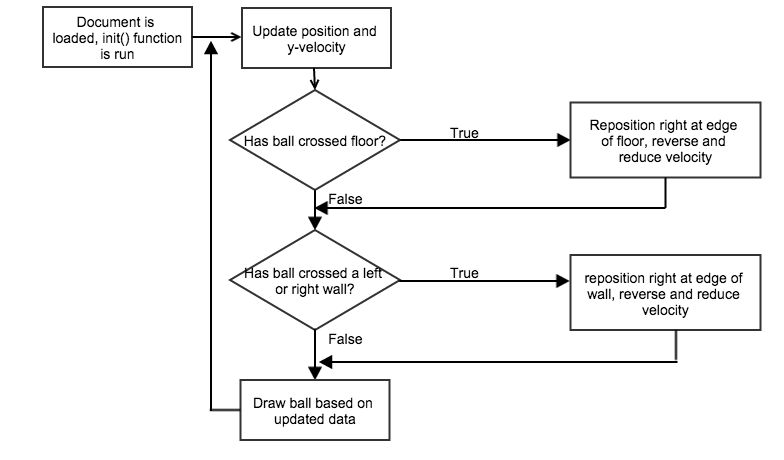
\includegraphics[width=15cm]{Figures/basicbouncingball.png}

	\caption{The logic flow chart of the basic bouncing ball simulation}
	\label{fig:basicbouncingball}
\end{figure}




\section{More Advanced Ball Bouncing}

While the previous example realistically incorporated the basic kinematic equations into account, it still fails to recognize important fundamentals of physics.  The simulation in this chapter will still be a simple ball bouncing, but will take into account air resistance.

\subsection{Background Physics}

Drag is generally defined as the force on an object that resists its motion through a fluid.  In the case of air resistance, the fluid is a gas, and therefore the process is called aerodynamic drag.  Most of the drag force results as a response to the inertia of the fluid: the resistance it exerts to oppose being pushed aside.  This can be expressed in the equation below:

\begin{equation} \label{eq:drag}
f_{drag} = -\frac{1}{2}C_d \rho A v^2
\end{equation}

The equation involves a negative sign because the force of drag is always opposite the direction of motion.  $C_d$ is referred to as the drag coefficient, and is a dimensionless quantity that is used to model complex dependencies of shape, inclination, and flow conditions.  While $C_d$ is in general not an absolute constant for a given body shape, for the purpose of these simulations constant values were used.  These values are typically determined experimentally: for example, the $C_d$ of a sphere is approximately .47.  In equation \ref{eq:drag}, $\rho$ is the mass density of the fluid, in $\frac{kg}{m^3}$.  Most of the simulations in this thesis occur in air, which has a density of 1.225 $\frac{kg}{m^3}$  (at sea level and 15 \textdegree C).  Running the simulations in different fluids can be simulated by changing $\rho$ to higher values (water, for example, would have $\rho$ equal to 1000 $\frac{kg}{m^3}$).  Lastly, $A$ in equation \ref{eq:drag} is the cross-sectional area of the object.  A sphere, for example, would have a cross-sectional area of $\pi r^2 $ 

The basic kinematic equations can also be used to make the simulations more physically realistic.  

\begin{equation}\label{eq:position}
d = v_i t+ \frac{1}{2}at^2
\end{equation}
\begin{equation}\label{eq:v}
v_f = v_i + at
\end{equation}

These equations are fundamental to any physical situation and can be used to make the ball bouncing example of the previous section more realistic

\subsection{The Code}

Using these basic mechanics equations, the previous ball bouncing example can be made more physically accurate.  The code below shows a second simulation which incorporates air resistance:

\setstretch{1}
\begin{lstlisting}[breaklines=true, frame=single, numbers=left, caption=More advanced ball bouncing simulation, label=lst:ballbounce2]
var x = 40;
var y =40;
var vy = 0;
var ay = 0;
var m = 1;
var r = 20;
var rSI = r* 0.000230909;  // radius in SI, converting px to m
var C_r = .8;  // Coefficient of restitution (tennis ball would be .8)
var rho = 1.2;    // density of air would be 1.2, water would be 1000
var dt = 60/1000;  // Time Step
var C_d = 0.47; //Coefficient of drag for sphere
var A = Math.PI * rSI * rSI;
var color = 'red';

window.onload = init();
  
function init(){
  setInterval(onEachStep, 1000/60);
}

function onEachStep(){ 
  var fy = 0;
  fy += m * 9.81;   // weight force
  if (vy>=0){
    fy -= 1* 0.5 *rho * C_d *A *vy *vy; 
  } 
  else {
    fy += 1*0.5 *rho *C_d *A *vy *vy;
  }

  ay = fy / m;
  vy += ay * dt;
  y += vy;
  
  // simple collision detection for floor only
  if (y + r > canvas.height){ 
    vy *= -C_r; 
    y = canvas.height - r;  
  }
  drawBall();
}
\end{lstlisting}
\setstretch{2}

To eliminate redundancy, the code doesn't show previous functions used, such as drawBall().  The code also doesn't show the basic steps to initialize any simulation with the canvas and context commands.  The code is very similar to the simulation in the previous section, except it incorporates air resistance.  Essentially, this simulation uses more kinematic equations, by calculating the net force, acceleration, and velocity for each frame.  First, the net vertical force is caculated, by combining the force of gravity $F_g = mg$ with the air drag from equation \ref{eq:drag}.  This step involves a conditional loop for the cases of positive and negative velocity.  Once the net force is calculated, the acceleration in the y-direction is found by using Newton's 2nd law of $F = ma$.  From there, the velocity and vertical position of the ball are updated.  Unlike the previous simulation, this example involves a variable dt, which is set to $\sim$16 ms for the same 60 frames per second.   


This code involves interesting conversions between pixels and meters.  Becuase the on screen simulation is presented eventually in terms of pixels, the physics equations must acknowledge this.  The variable rSI on line 7 converts the radius of ball from pixels into meters.  This is accomplished knowing the pixel density of the screen.  This is commonly approximately 100 (dots per inch).  The simulations were optimized for a macbook pro 15 inch model, which features 110 dpi.  The calculation is shown below:

\begin{equation}\label{eq:pixels}
\frac{1m}{100 cm} \hspace{1mm} \frac{2.54 cm}{1 in}  \hspace{1mm}   \frac{1 in}{110 px} \approx  0.00023091 \frac{m}{px}
\end{equation}

Once the conversion is made, the physics equations use the radius of the ball in terms of meters instead of pixels, which would give erroneous answers.

\section{Multiple Balls Bouncing}

So far, this chapter has dealt with a single object in motion.  However, physics rarely involves just one body in motion.  To demonstrate how more than one object can be displayed simultaneously, this section will show the case of multiple bouncing balls.  There is no new physics introduced in this section, but the coding concepts will be used repeatedly in later chapters of this thesis.

\subsection{The Code}

To generate more than one object, arrays can be used.  The code below relies on arrays and object prototypes to create the effect:

\setstretch{1}
\begin{lstlisting}[breaklines=true, frame=single, numbers=left, caption=Multiple balls bouncing simulation, label=lst:ballsbouncing]
var g = 0.1635;
var balls;
var numBalls = prompt('how many balls would you like to have bounce?'); 
var C_d = .8;
 
window.onload = init; 
 
function init() {
  balls = []; // creates empty array
  for (var i=0; i<numBalls; i++){
    radius = Math.random()*20+5;
    var ball = new Ball();  
    ball.x = 50;
    ball.y = 75;
    ball.radius =  radius;
    ball.vx = Math.random()*15;
    ball.vy = (Math.random()-0.5)*10;
    ball.color = getRandomColor();
    ball.draw(context);
    balls.push(ball);
  }  
  setInterval(onEachStep, 1000/60); // 60 fps
};
 
function onEachStep() {
  context.clearRect(0, 0, canvas.width, canvas.height); 
  for (var i=0; i<numBalls; i++){
    var ball = balls[i];
    ball.vy += g;     

    if (ball.vx >0){ // while vx is positive, decrease to show friction/air drag
    ball.vx -= .001;
  } else{
    ball.vx === 0;// make sure ball stops moving appropriately
  }
    ball.x += ball.vx; 
    ball.y += ball.vy; 
      
    if (ball.y > canvas.height - ball.radius){ 
      ball.y = canvas.height - ball.radius; 
      ball.vy *= -C_d; 
    }
    if (ball.x + ball.radius > canvas.width){
      ball.x = canvas.width - ball.radius; 
      ball.vx *= -C_d;
    }
    if (ball.x < ball.radius){
      ball.x = ball.radius;
      ball.vx *= -C_d;
    }
    ball.draw(context); 
  } 
};

function getRandomColor() {
    var letters = '0123456789ABCDEF'.split('');
    var color = '#';
    for (var i = 0; i < 6; i++ ) {
        color += letters[Math.floor(Math.random() * 16)];
    }
    return color;
}
\end{lstlisting}
\setstretch{2}


As with previous code listings, steps outlined in previous examples have been omitted to save space.  This code differs mainly from previous examples because of its usage of prototypes, objects, and arrays.  A separate javascript file, ball.js, contains the framework code for creating a ball.  This will be used more in future chapters, so the code doesn't have to be repeated.  This function is called a constructor function, becuase it allows other parts of code to reference the function when creating a new object.  In the case of listing \ref{lst:ballsbouncing}, an array holds an object for each different ball generated.  The number of elements in the array is equal to the number of balls, which is selected by the user through the prompt() method on line 3.  The object in each array element contains different properties for each ball: the radius, color, position, and velocities.  For every frame of the simulation, a loop cycles through each element of the balls array, changing the properties of position and velocity, on lines 29 and 36-37.  Exactly like in section 1, there is a conditional loop that controls the event of the ball colliding with a wall.  The logic of this program can be visualized in the flow chart of figure \ref{blah}.

Because of repeated for loops, this program involves a bit more complexity than the previous examples.  However, the physics is very simple in this case.  Future chapters will combine more complex physics with this complexity of coding to create more advanced simuations.  These simulations can put a strain on a computer's performance: to simulate 20 balls bouncing, at 60 frames per second, 4,800 individual properties of objects need to be generated each second.  Luckily, with the modern capabilities of computers, this isn't too difficult.  

This program involves each ball having a random color and radius, when the balls array is created in the init() function.  The Math.rand() method is used for both of these, and is fundamental to the other simulations in this thesis.  The random color generator function operates by creating a hex color by randomly assigning the 16 possible entries to each entry of the 6 character string.  While completely unnecessary, this gives the program aesthetic appeal, and makes it easier to distinguish the balls.

\begin{figure}[t]  
  \centering
  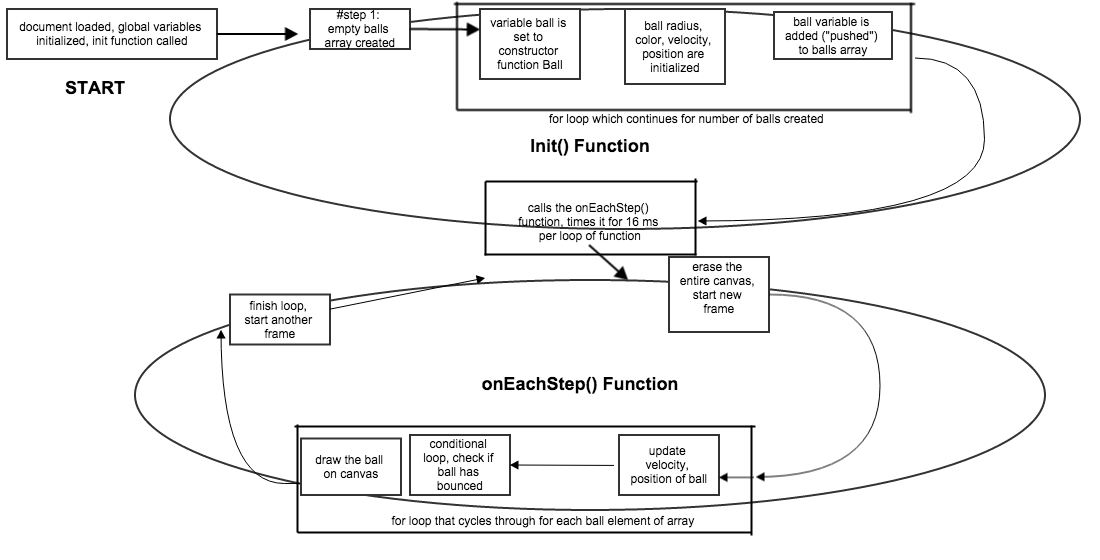
\includegraphics[width=15cm]{Figures/ballsbouncing.png}
  \caption{The logic flow chart of the balls bouncing simulation}
  \label{blah}
\end{figure}






































% Chapter 2

\chapter{Simulating Orbits} % Main chapter title

\label{Chapter2} % For referencing the chapter elsewhere, use \ref{Chapter1} 

\lhead{Chapter 2. \emph{Simulating Orbits}} % This is for the header on each page - perhaps a shortened title

%----------------------------------------------------------------------------------------

In this chapter, a more advanced simulation of orbiting masses will be introduced.  First, a simple orbit situation will be introduced, followed by more complex examples involving escape velocities.  While the physics still isn't too advanced, the coding necessary is a bit more challenging.  



\section{Basic Orbit Path}

The first simulation will deal with an example of a planet orbiting another much more massive planet.  

\subsection{Background Physics}



This entire chapter is centered around Newton's law of universal gravitation:

\begin{equation}\label{universalgravity}
F_g = G \frac{m_1 m_2}{r^2} 
\end{equation}

Where $F_g$ is the magnitude of the force acting on either mass, G is the gravitational constant ( SI units of $6.67 \hspace{1mm} \frac{Nm^2}{kg^2}$ ), $m_1$ is the mass of one object, $m_2$ is the mass of the other object, and $r$ is the radius separating the two masses.  By Newton's 3rd law, there is an equal and opposite force exerted on each mass.  

This equation can be used to describe the orbiting paths of planets.  For simple cases when one planet orbits another, the variables m and M can be used.  For a first example, we will assume M \textgreater \textgreater  m, that is, one planet has a much greater mass than the other.  Therefore, while each planet exerts an equal force on the other, the acceleration on the massive planet will be negligible.  So, the smaller planet will orbit around the stationary planet, without attracting the larger planet enough to move it.  




\subsection{The Code}  

The full code is shown in the listing below:

\setstretch{1}
\begin{lstlisting}[breaklines=true, frame=single, numbers=left, caption=Basic planet orbiting simulation, label=lst:basicorbit]
var canvas = document.getElementById('canvas');
var context = canvas.getContext('2d'); 
var canvas_bg = document.getElementById('canvas_bg');
var context_bg = canvas_bg.getContext('2d');

var planet;
var sun;
var m = 1; // planet's mass
var M = 1000000; // heavy planet's mass
var G = 1;
var t0,dt;

window.onload = init; 

function init() {
	// create a stationary large planet
	sun = new Ball(70,'orange',M);
	sun.pos2D = new Vector2D(275,200);	
	sun.draw(context_bg);
	// create a moving planet			
	planet = new Ball(10,'blue',m);
	planet.pos2D = new Vector2D(200,50);
	planet.draw(context);
	// make the planet orbit the large planet
	t0 = new Date().getTime(); 
	animFrame();
};

function animFrame(){
	animId = requestAnimationFrame(animFrame,canvas);
	onTimer(); 
}
function onTimer(){
	var t1 = new Date().getTime(); 
	dt = 0.001*(t1-t0); 
	t0 = t1;	
	if (dt>0.1) {dt=0;};	
	move();
}
function move(){			
	moveObject(planet);
	calcForce();
	updateAccel();
	updateVelo(planet);
}

function moveObject(obj){
	obj.pos2D = obj.pos2D.addScaled(obj.velo2D,dt);	
	context.clearRect(0, 0, canvas.width, canvas.height);
	obj.draw(context);	
}
function calcForce(){
	force = Forces.gravity(G,M,m,planet.pos2D.subtract(sun.pos2D));	
}	
function updateAccel(){
	acc = force.multiply(1/m);
}	
function updateVelo(obj){
	obj.velo2D = obj.velo2D.addScaled(acc,dt);				
}
\end{lstlisting}
\setstretch{2}

This program differs from previous ones used so far in that it uses two canvases instead of one.  This is essential for having the large planet remain stationary and not being erased every frame.  Instead, there can be a constant ``background'' canvas containing the stationary planet.  The code begins by initializing the variables planet and sun, where sun simply refers to any large planet that has much more mass.  The gravitational constant $G$ is intialized as a formality just to a value of 1.  G in this simulation isn't necessary, because the constant simply is used for unit conversion.  This will become clear later in this section.  When the web page is loaded, it calls the init function, just as in previous simulations.  The init function creates the sun and planet as objects from the Ball constructor function, exactly as in chapter 1.  Instead of having separate variables x and y in the previous examples, the position information can be stored into a property of each object, which is created using a different constructor function Vector2D.  

The next function, animFrame, functions simply by initializing the javascript animation frame, and then calling the next function, onTimer.  This next function creates a variable dt by converting the unit javascript operates in (ms) to SI units of s.  It then passes the flow of the program onto the next function, move.  This function involves calling 4 functions, the first of which simply updates the position of the planet, erases the foreground canvas, and then draws the updated canvas.  This step can be analyzed through a physics kinematics equation:

\begin{equation}\label{velo}
x(t+dt) = x(t) + v_x(t)dt
\end{equation}

This is essentially analagous to Euler's method, by understanding that $v_x = \frac{dx}{dt}$.  

\begin{equation}\label{euler}
x(t+dt) = x(t) + \frac{dx}{dt}\left(0\right) dt
\end{equation}

By using constructor functions, with 2 different properties for the x and y position, the planet's location can be updated without updating variables and taking up more space.  The location has to be updated for every frame, but so does the force, acceleration, and velocity.  These next 3 steps are the remaining functions of the move function.  The calcForce function updates the force of gravity acting on the planet, using equation \ref{universalgravity}.  This equation calculates r by calculating the displacement vector between the two planets, and finding the magnitude of that vector.  The updateAccel function simply takes the updated force vector and scales it by a certain ``k'' value which is represented by dividing by the mass.  This is the step that incorporates Newton's 2nd law of $a = \frac{F}{m} $.  The last function updates the velocity of the planet, similar to how the position was updated.  Using Euler's method like before, we come to the following equation

\begin{equation}\label{euleraccel}
 v (t+dt) =  v(t) + a(t)dt 
\end{equation}





Essentially, what makes this program more complicated is that it uses many other functions to accomplish the overall simulation.  However, this method of programming makes future simulations easier--the same functions can be used, with changed variables.  The code listing below shows these ``tool'' functions that are used in future chapters of this thesis:

\setstretch{1}
\begin{lstlisting}[breaklines=true, frame=single, numbers=left, caption=Various tools functions used for orbit simulation, label=lst:basicorbittools]
function Vector2D(x,y) {
	this.x = x;
	this.y = y;		
}	
Vector2D.prototype = {		
	lengthSquared: function(){
		return this.x*this.x + this.y*this.y;
	},
	length: function(){
		return Math.sqrt(this.lengthSquared());
	},
	add: function(vec) {
		return new Vector2D(this.x + vec.x,this.y + vec.y);
	},
	subtract: function(vec) {
		return new Vector2D(this.x - vec.x,this.y - vec.y);
	},
	multiply: function(k) {
		return new Vector2D(k*this.x,k*this.y);
	},
	addScaled: function(vec,k) {
		return new Vector2D(this.x + k*vec.x, this.y + k*vec.y);
	},	

	function Forces(){
}
Forces.gravity = function(G,m1,m2,r){
	return r.multiply(-G*m1*m2/(r.lengthSquared()*r.length()));
}
\end{lstlisting}
\setstretch{2}


\section{Escape Velocity}

The previous section tested situations where the planet orbited the sun continuously.  However, if the speed is great enough, the orbiting body is capable of ``escaping'' from the larger planet's influence.  The minimum speed necessary for this is called the escape velocity.  

This can be derived by understanding conversation of energy.  When an object leaves the surface of a planet, it will have an initial kinetic energy, and potential gravitational energy.  This will equal the final potential energy, defined as a condition when the final kinetic and gravitational potential energy is 0.  This relationship is shown in the equation below:

$$K_i + U_{g_{i}} = K_f + U_{g_{f}}$$

Knowing that the final kinetic and gravitational energy is 0, this equation becomes:

$$\frac{1}{2}mv_{esc}^2 - \frac{GMm}{r} = 0 + 0  $$

Solving for $v_{esc}$ yields the following:

\begin{equation}\label{eq:escapevelocity}
v_{esc} = \sqrt{\frac{2GM}{r}}
\end{equation}

Where G is the gravitational constant, M is the mass of the planet the object is escaping from, and r is the starting distance from the center of mass of the planet.  

To test the physics behind the escape velocity, a slightly different scenario can be created with a different program.  This simulation will have the object begin right at the surface of the larger planet, to emulate the process of ``escaping'' from the planet's gravity influence.  To visualize this, a much larger canvas will be used, and some code changes will be utilized, seen below:


\setstretch{1}
\begin{lstlisting}[breaklines=true, frame=single, numbers=left, caption=New conditions for escape velocity simulation, label=lst:changestoorbit]
sun = new Ball(400,'orange',M);
sun.pos2D = new Vector2D(

planet = new Ball(10,'blue',m);
planet.pos2D = new Vector2D(500,2490);

planet.velo2D = new Vector2D(0, -80);
\end{lstlisting}
\setstretch{2}

These changes made the larger planet look visually bigger, to simulate the effect of a massive planet.  It also positioned the object to begin right on the surface of the larger planet (in this case, 410 pixels above the center of mass of the larger planet).  To calculate the escape velocity for the situation above, equation \ref{eq:escapevelocity} can be used, but understanding some key factors:

\begin{enumerate}
\item The escape velocity calculated will be in $\frac{px}{s}$ instead of SI unit $\frac{m}{s}$
\item The masses of each planet don't need to contain units, it can more just represent a ratio between the large and small planet.  Therefore, each mass will be a unitless quantity, just used as a test of the escape velocity equation.
\item Similarly to  \#2, the gravitational constant G doesn't have to include units, since this test is only in a more theoretical sense, and doesn't use actual units of mass.  However, using dimensional analysis, for the equation below to make sense, G could be viewed as having units of $\frac{px^3}{s^2}$.
\end{enumerate}

Proceeding with these conditions in mind, the escape velocity for the simulation of code listing \ref{lst:updatedorbit}
can be calculated as shown below:

\begin{equation}\label{eq:calcvescape}
 v_{esc} = \sqrt{\frac{2*1 \frac{px^3}{s^2}*1000000}{410 px}} \approx 69.843 \frac{px}{s} 
\end{equation}

Therefore, with the program simulation, any initial speed greater than this value will escape the gravitational influence of the larger planet.  To test this, I used the following code to print out values of the velocity continuously:

\setstretch{1}
\begin{lstlisting}[breaklines=true, frame=single, numbers=left, caption=Code for printing out values of speed, label=lst:changestoorbit]
var i =0;
i++;
if(i%15 ===0){console.log(planet.velo2D.length());}
\end{lstlisting}
\setstretch{2}

This code operates by printing out the value of the speed of object 4 times per second, understanding that i is incremented by 1 for each frame, and there are the usual 60 frames per second.  The data is outputted through the console.log() method, which prints it onto the web browser.  This data was then plotted for different initial speeds, and the results are shown below:


\begin{figure}[h] 
	\centering
		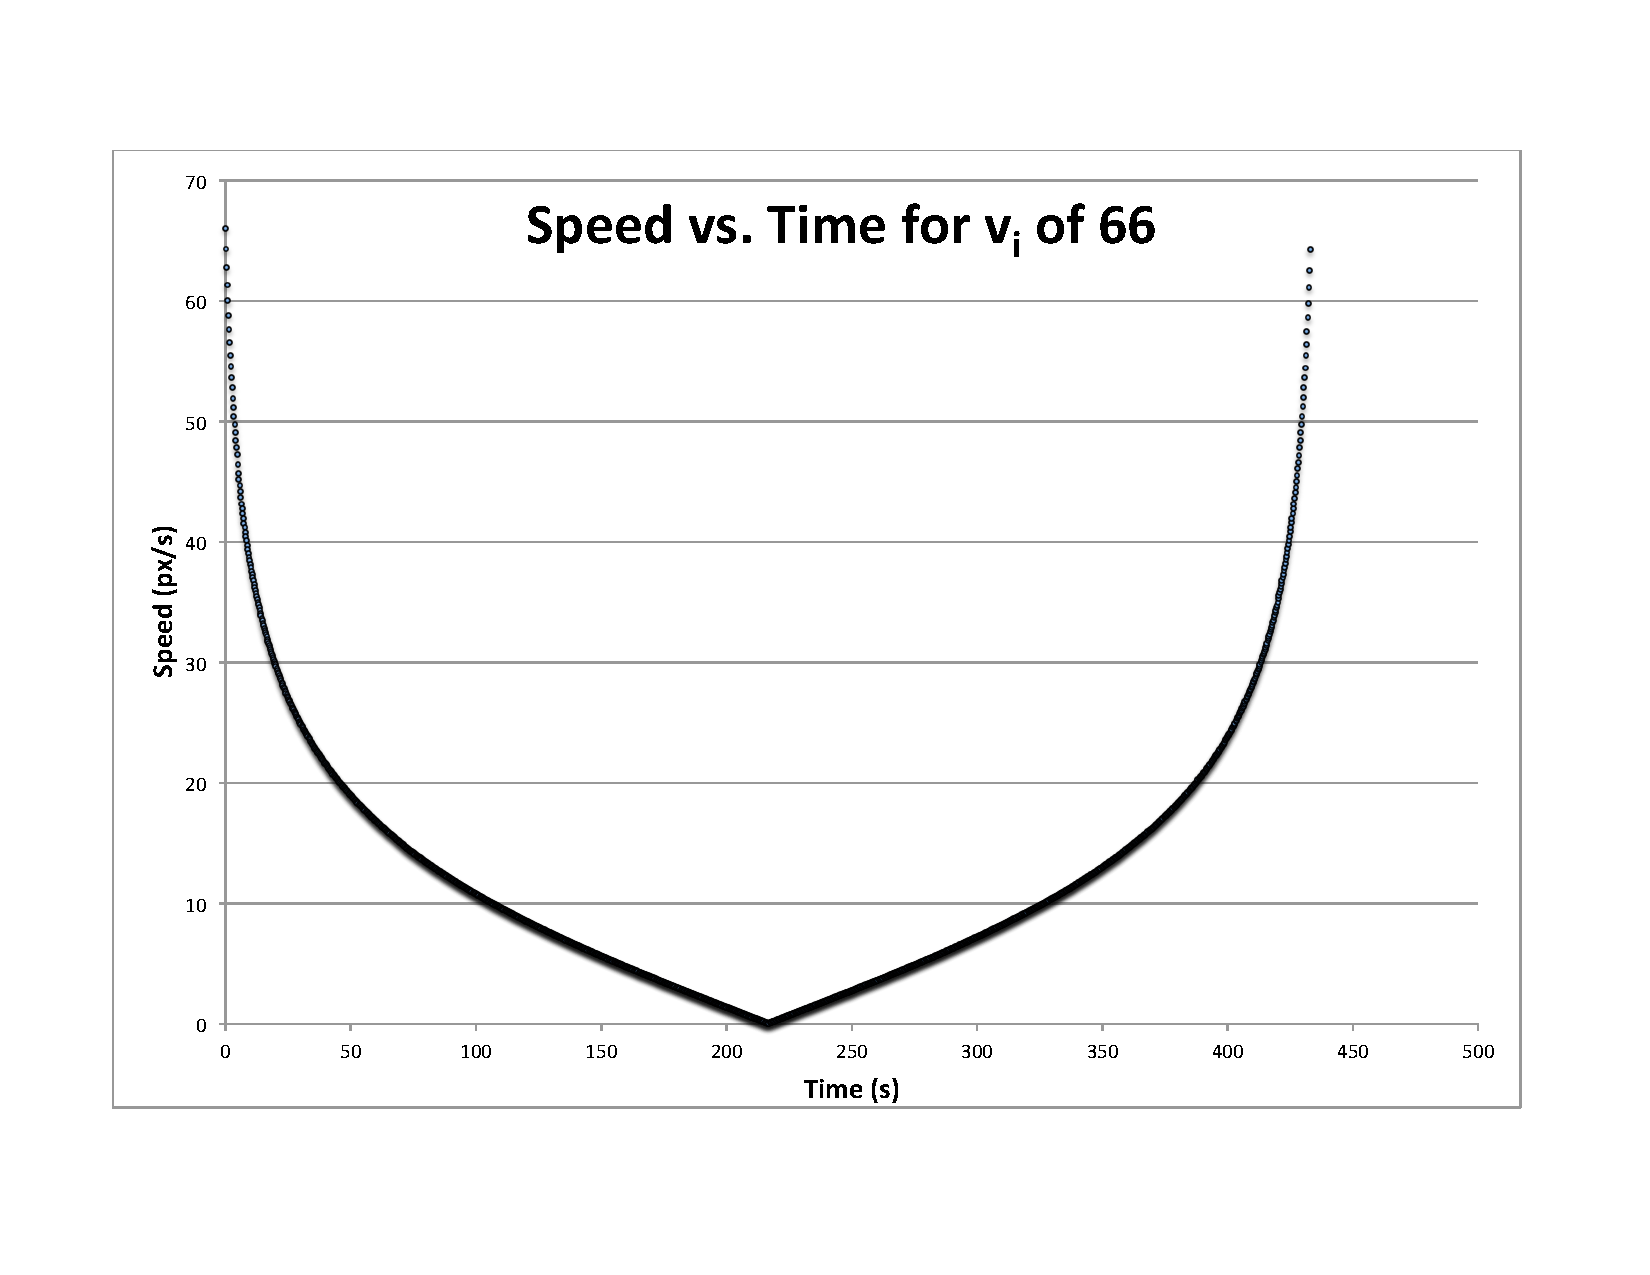
\includegraphics[width=12cm]{Figures/fig1.pdf}

	\caption{Speed vs. time for initial $v_i$ of 66 $\frac{px}{s}$}
	\label{fig:data1}
\end{figure}


\begin{figure}[h] 
	\centering
		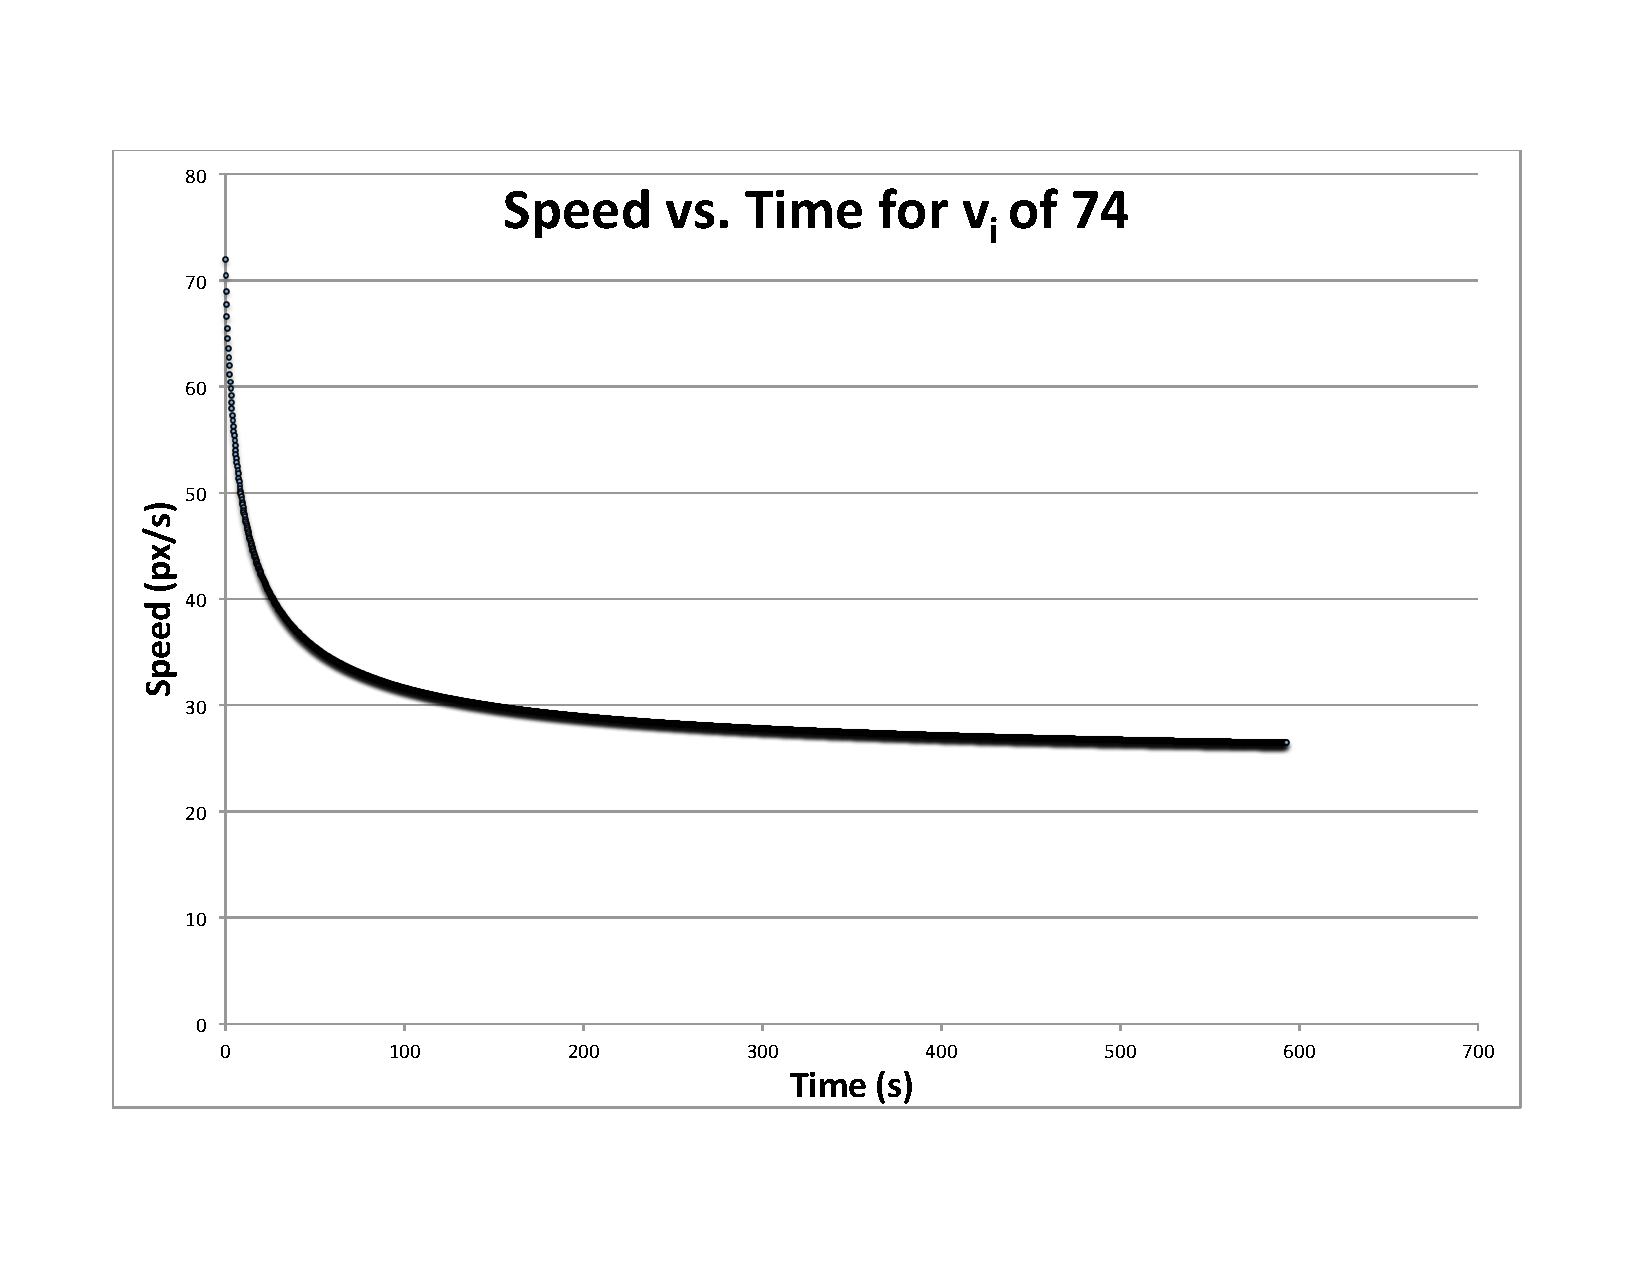
\includegraphics[width=12cm]{Figures/fig2.pdf}

	\caption{Speed vs. time for initial $v_i$ of 74 $\frac{px}{s}$}
	\label{fig:data2}
\end{figure}


\begin{figure}[h] 
	\centering
		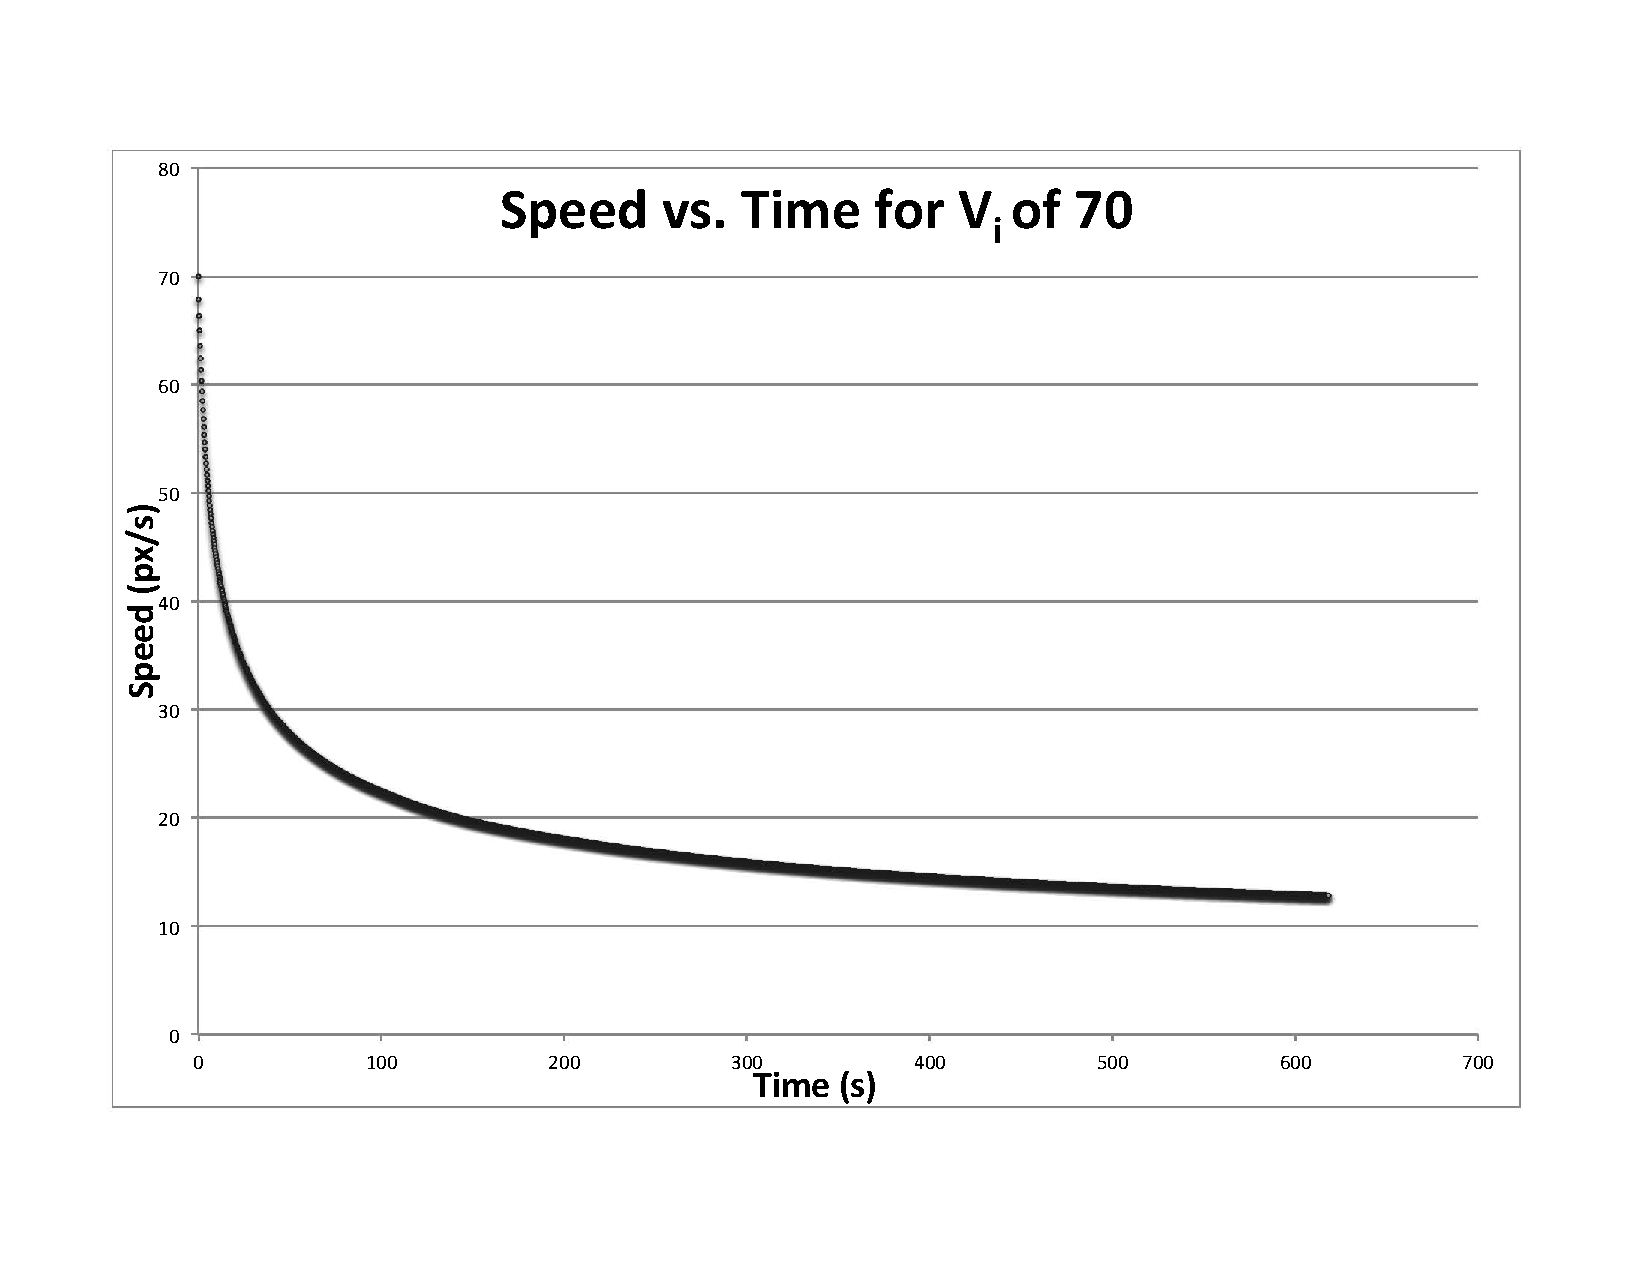
\includegraphics[width=12cm]{Figures/fig3.pdf}

	\caption{Speed vs. time for initial $v_i$ of 70 $\frac{px}{s}$}
	\label{fig:data3}
\end{figure}



These 3 figures show the stuff that happens with differet velocitias.  need to talk about how near the escape velocity, intersting things happen.  obvious results would occur far away from it.

These 3 figures show the speed vs. time for different intial velocities.  Figure \ref{fig:data1} shows an initial speed of 66, which isn't enough for the required 69.843 speed to leave the influence of the larger planet.  The object rises far away from the planet, slows down, and then reaches a point where the speed is 0, and then reverse direction and accelerates back towards the planet.  Figures \ref{fig:data2} and \ref{fig:data3} show initial speeds greater than that of the escape velocity, and the effect is clear: the speed tapers off eventually to an end velocity, as r approaches $\infty$ and the gravity force approaches 0.  If the initial speed exactly equaled the escape velocity, in theory the final speed of the object would approach 0, and r approaches $\infty$.  However, this simulation would take a very long time to do.  All of these graphs were plotted over times ranging from 400 to 700 seconds, and since the speed was printed 4 times per second by the computer program, there were thousands of data points plotted overall. 





\section{Kepler's Laws}




In the early 1600's Johannes Kepler proposed a series of laws that explained how planets orbit the sun.  This was the support the scientific-based heliocentric model, which conflicted with the geocentric model before that.  These 3 laws are shown below:



\begin{enumerate}
\item All planets move in ellpitical orbits with the Sun at one focus
\item The radius vector drawn from the Sun to a planet sweeps out equal areas in equal time intervals
\item The square of the orbital period of any planet is proportional to the cube of the semimajor axis of the elliptical orbit
\end{enumerate}

The simulation in this section will help visualize law \#2, using the orbit program already created in section 2.1  This law can be derived by understanding the situation of a planet orbiting the sun in an ellpitical.  The sun is assumed to be much more massive so it doesn't move.  At any instant along the path of orbit, the planet has a gravitational force pointing towards the sun, and it's velocity is tangential to this inward force.  This can be visualized in figure \ref{fig:sun1}.  

\begin{figure}[h] 
	\centering
		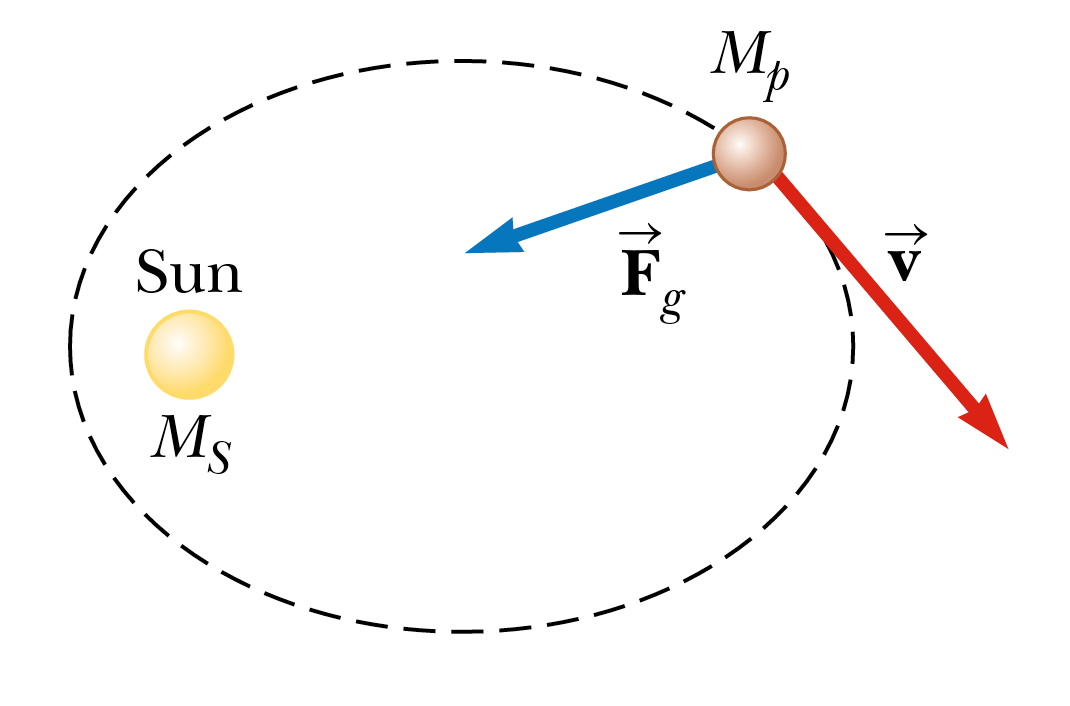
\includegraphics[width=8cm]{Figures/sun1.png}
	\caption{Basic model of planet orbiting a sun}
	\label{fig:sun1}
\end{figure}


The gravitational force is a central force that always points antiparallet to the radius vector $\vec{r}$.  Knowing the radius vector and force on the planet at any point, the torque can be calculated, from the equation below:

\begin{equation}\label{eq:torque}
\vec{\tau} = \vec{r}\times\vec{F_g} = \frac{d\vec{L}}{dt}
\end{equation}


Because the radius and force vector are always antiparallel to one another, the torque, and therefore, the change in angular momentum will equal 0.  In other words, $\vec{L}$ will remain constant.  Knowing that $\vec{p} = M_p \times \vec{v}$, the following can be derived:

$$ \vec{L} = \vec{r}\times \vec{P} = M_p \vec{r}\times\vec{v}  $$

However, since the angle between $\vec{r}$ and $\vec{v}$ is always 90\textdegree, the equation above can expressed as:


\begin{equation}\label{eq:torquederive}
L = M_p \left|\vec{r} \times \vec{v}\right|
\end{equation}

This equation can be related to figure \ref{fig:sun2}, which shows the relationship between $\vec{r}$ and $d\vec{r}$.

\begin{figure}[h] 
	\centering
		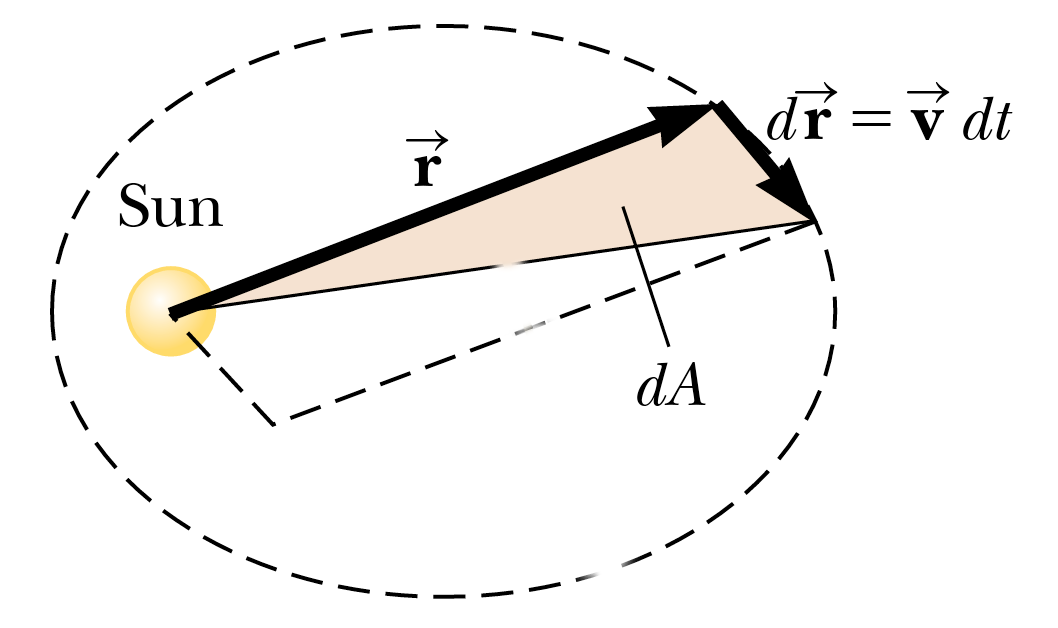
\includegraphics[width=8cm]{Figures/sun2.png}
	\caption{Relationship between  $\vec{r}$ and $d\vec{r}$}
	\label{fig:sun2}
\end{figure}

$\vec{r} \times d\vec{r}$ equals the area of the parallelogram in figure \ref{fig:sun2}.  As $dt \rightarrow  0$, the area $dA$ equals $\frac{1}{2}$ the area of this same parallelogram.  Using this relationships yields the following:

$$ dA = \frac{1}{2}|\vec{r} \times d\vec{r}| = \frac{1}{2}\left|\vec{r} \times \vec{v} dt \right| = \frac{1}{2}\left|\vec{r} \times \vec{v}\right| dt  $$

Rearranging equation  to solve for $\left|\vec{r} \times \vec{v}\right|$, and substituting this into the above expression yields the following:

$$ dA = \frac{1}{2}\left(\frac{L}{M_p}\right)dt  $$

Finally, dividing both sides by dt yields the final equation:

\begin{equation}\label{dadt}
\frac{dA}{dt} = \frac{1}{2}\left(\frac{L}{M_p}\right)
\end{equation}

Since $L$ and $M_p$ are constants, this equation shows that the rate of change in area is constant.  To visualize this, slight adjustments were made to the simulation of section 1.  The code changes are shown below:



\setstretch{1}
\begin{lstlisting}[breaklines=true, frame=single, numbers=left, caption=Code for printing out values of speed, label=lst:changestoorbit]
if(i<960){
	if(i%30===0){
	context.strokeStyle = 'white';
	context.moveTo(planet.x, planet.y);
	context.lineTo(sun.x, sun.y);
	context.stroke();
	var dr = Vector2D.distance(planet.pos2D, planet.oldpos2D);
	var r =  Vector2D.distance(planet.pos2D, sun.pos2D);
	console.log('dA is equal to:  %f', .5*r*dr);
	planet.oldpos2D=planet.pos2D;
	}
\end{lstlisting}
\setstretch{2}

This code creates a condition where ever .5 seconds, a line is drawn between the position of the sun and the position of the planet.  This visualizes the display of breaking up the orbit path into different area segments, which should all be equal area.  Because the simulation occurs at a consistent rate of 60 frames per second, the lines could be drawn at a consistent rate over time.  The code also calculates a variable r, which is the magnitude of the displacement vector between the two positional vectors of the planet and sun.  The vector dr is also calculated by comparing the positional vectors of the planet between two different times.  With these two variables, the program performs a rough calculation of dA, by understanding it is approximately $\frac{1}{2}$ the area of the parallelogram.  The areas were the same within a reasonable amount of uncertainty and accuracy possible with the javascript program.  The smallest ``dt'' possible in this program is 17 ms due to the limitations of the animation method of javascript.  However, if dt could be made to approach 0, the calculations of dA would likely be closer to one another.

A screenshot of the simulation is shown below for reference:

\begin{figure}[h] 
	\centering
		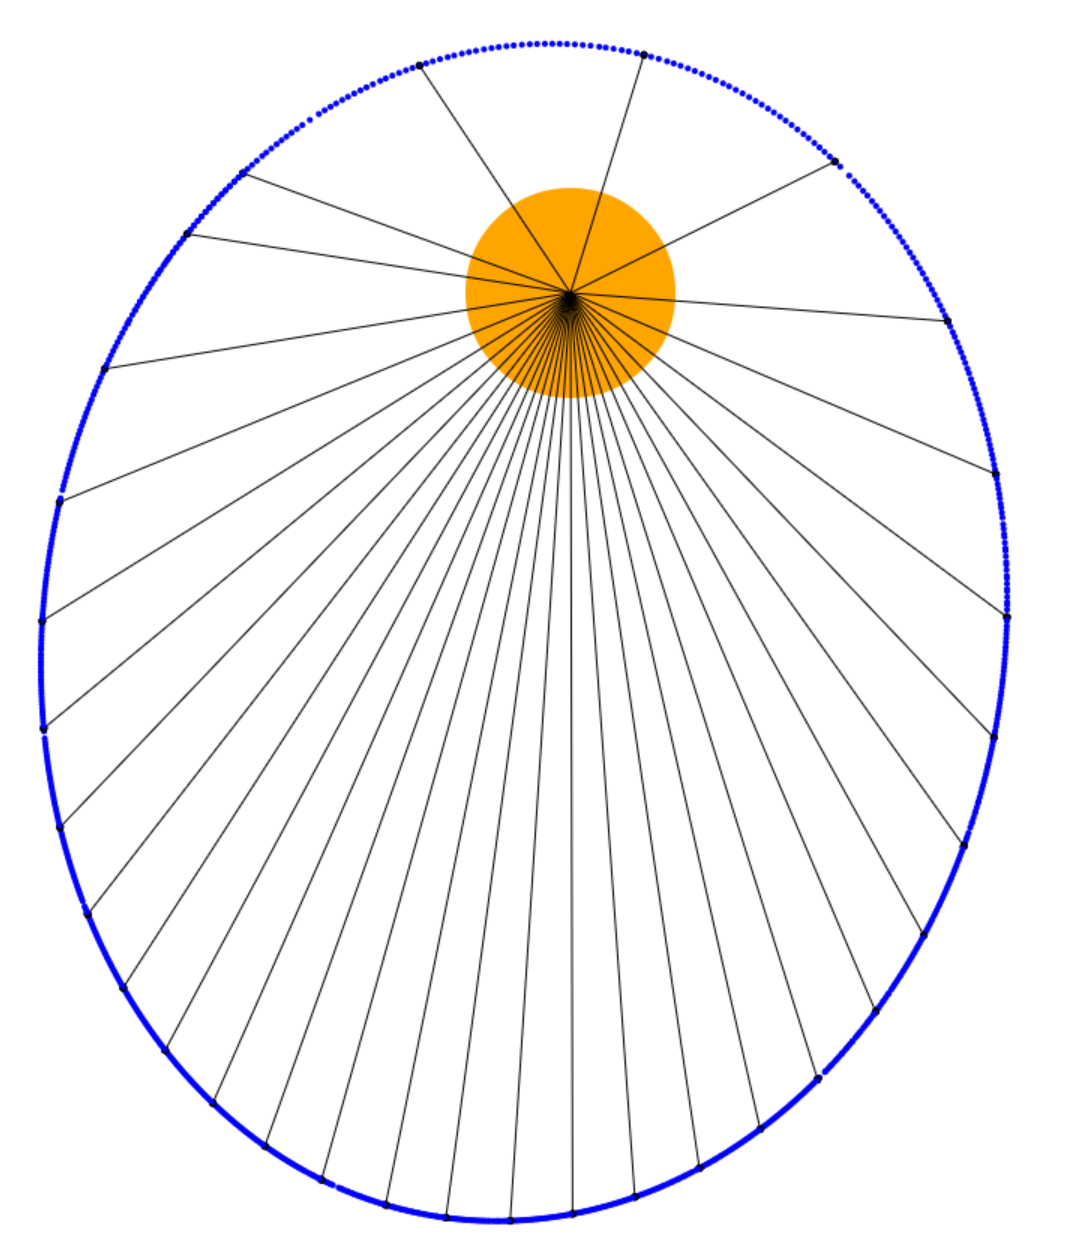
\includegraphics[width=7cm]{Figures/keplerscreenshot.png}
	\caption{Screenshot of kepler law test simulation}
	\label{fig:sun1}
\end{figure}

The screenshot helps visually understand Kepler's 2nd law by separating areas of the same change in time by lines.





























 
% Chapter 3

\chapter{Rigid Body Motion} % Main chapter title

\label{Chapter3} % For referencing the chapter elsewhere, use \ref{Chapter1} 

\lhead{Chapter 3. \emph{Rigid Body Motion}} % This is for the header on each page - perhaps a shortened title

%----------------------------------------------------------------------------------------

Previous chapters have disregarded rotational motion of solid bodies.  This chapters examines the mechanics of rigid body rotations and collisions through angular momentum fixed axis rotation.  Simulations will involve rigid body collisions.


\section{Background Physics}

Previous sections in this thesis have simply involved translational motion.  The theorem of rigid body motion states that the displacement of any rigid body can be decomposed into two independent motions: the translation of the center of mass, and the rotation about the center of mass.  A rigid body in general is defined as an object that maintains its shape and size when a force is applied to it.  In reality, all objects experience some level of deformation, however for the purpose of these simulations it is safe to ignore this.    



% Conclusion

\chapter{Conclusion} % Main chapter title

\label{Conclusion} % For referencing the chapter elsewhere, use \ref{Chapter1} 

\lhead{Conclusion} % This is for the header on each page - perhaps a shortened title

%----------------------------------------------------------------------------------------

\setstretch{2}
Physics simulations can be made highly realistic through JavaScript.  This thesis only presents a few of the many possibilities.  The methods of programming applied in this thesis can be summarized in a few simple steps:

\begin{enumerate}  
\item Initialize global variables and constants
\item Initialize the repetitive loop of animation, in a variety of different ways
\item Prepare conditions to be updated on each frame of animation, such as position, speed, acceleration or force
\item Draw the current conditions to the canvas, and then erase the canvas to give the illusion of motion
\end{enumerate} 

By providing specific rules of code for each frame of the simulation, the program can emulate realistic physics processes.  The simulations can easily be edited to allow for many different situations.  This is the main advantage of simulations as opposed to video animations that can't be edited easily once created.     


These simulations can be made more advanced and complex if they are incorporated in three dimensions.  This can be done by utilizing web GL, a JavaScript API which is used to render 3D objects in the canvas.  If I had more time or worked on a full-year thesis, I would look to expand these simulations into more advanced 3D simulations.  Much of the physics of chapter 3 doesn't take into account the vector $\vec{k}$ simply because the simulations in this thesis only involved $\vec{i}$ and $\vec{k}$.  


The most challenging part of this thesis was overcoming small JavaScript bugs that occurred.  I had to invest considerable time at the beginning of the thesis to sharpen my JavaScript skills.  Sometimes the code confused me when using multiple different functions, based from different prototypes.  Chapter 3 was also challenging for me to apply the mechanics concepts to actual code.  These types of simulations have a wide variety of real world applications, and I have enjoyed the opportunity to expand my understanding of physics concepts in this manner.

































 





%\input{Chapters/Chapter5} 
%\input{Chapters/Chapter6} 
%\input{Chapters/Chapter7} 





%----------------------------------------------------------------------------------------
%	THESIS CONTENT - APPENDICES
%----------------------------------------------------------------------------------------

\addtocontents{toc}{\vspace{2em}} % Add a gap in the Contents, for aesthetics

\appendix % Cue to tell LaTeX that the following 'chapters' are Appendices

% Include the appendices of the thesis as separate files from the Appendices folder
% Uncomment the lines as you write the Appendices

% Appendix A

\chapter{Full Code Listings From Ch. 1} % Main appendix title

\label{AppendixA} % For referencing this appendix elsewhere, use \ref{AppendixA}

\lhead{Appendix A. \emph{Full Code Listings From Chapter 1 }} % This is for the header on each page - perhaps a shortened title

\section{Simulation \#1:  Simple Ball Bouncing}

\setstretch{1}
\begin{lstlisting}[breaklines=true, frame=single, numbers=left, caption=A basic ball bouncing simulation, label=lst:ballbounce1]
var canvas = document.getElementById(`canvas');
var context = canvas.getContext(`2d'); 

canvas.height = screen.height-200;
canvas.width = screen.width -100;

var radius = 20;
var color = ``red";
var g = .1635; // acceleration due to gravity
var x = 40;  // initial horizontal position
var y = 40;  // initial vertical position
var vx = parseFloat(prompt(`what is the initial horizontal speed of ball you would like?(recommended values of 1-20'));  // initial horizontal speed 
var vy = 0;  // initial vertical speed
 
window.onload = init; 
 
function init() {
  setInterval(onEachStep, 1000/60); // 60 fps
};
 
function onEachStep() {
  vy += g; // gravity increases the vertical speed
  x += vx; // horizontal speed increases horizontal position 
  y += vy; // vertical speed increases vertical position

  if (y > canvas.height - radius){ // if ball hits the ground
    y = canvas.height - radius; // reposition it at the ground
    vy *= -0.8; // then reverse and reduce its vertical speed
  }
  if (x > canvas.width - radius){ // if ball hits right wall
    x = canvas.width - radius; // reposition it right at wall 
    vx *= -0.8;  // then reduce and reverse horizontal speed
  }
  if (x < radius){  // if ball hits left wall
    x = radius;  // reposition it right at wall
    vx *= -0.8  // then reverse and reduce horizontal speed
  }
  drawBall(); // draw the ball
};
 
function drawBall() {
  with (context){
    clearRect(0, 0, canvas.width, canvas.height); 
    fillStyle = color;
    beginPath();
    arc(x, y, radius, 0, 2*Math.PI, true);
    closePath();
    fill();
  };
};
\end{lstlisting}

\section{Simulation \#2: More Advanced Ball Bouncing}

\begin{lstlisting}[breaklines=true, frame=single, numbers=left, caption=More Advanced Ball Bouncing Simulation label=lst:ballbounce2]
var canvas = document.getElementById('canvas');
var context = canvas.getContext('2d');

canvas.height=screen.height-300;
canvas.width=screen.width-100;

var x = 40;
var y =40;
var vy = 0;
var ay = 0;
var m = 1;
var r = 20;
var rSI = r* 0.0002309090909;  // radius in SI, converting px to m
var C_r = .8;  // Coefficient of restitution (tennis ball would be .8)
var rho = 1.2;    // density of air would be 1.2, water would be 1000
var dt = 60/1000;  // Time Step
var C_d = 0.47; //Coefficient of drag for sphere
var A = Math.PI * rSI * rSI;
var color = 'red';

window.onload = init();
  
function init(){
  console.log(vy);
  setInterval(onEachStep, 1000/60);
}

function onEachStep(){ 
  var fy = 0;
  fy += m * 9.81;   // weight force
  if (vy>=0){
    fy -= 1* 0.5 *rho * C_d *A *vy *vy; 
  } 
  else {
    fy += 1*0.5 *rho *C_d *A *vy *vy;
  }

  ay = fy / m;
  vy += ay * dt;
  y += vy;
  
  // simple collision detection for floor only
  if (y + r > canvas.height){ 
    vy *= -C_r; 
    y = canvas.height - r;  
  }
  drawBall();
}

function drawBall() {
  with (context){
    clearRect(0, 0, canvas.width, canvas.height); 
    fillStyle = color;
    beginPath();
    arc(x, y, r, 0, 2*Math.PI, true);
    closePath();
    fill();
  };
};
\end{lstlisting}

\section{Simulation \#3: Multiple Balls Bouncing}

\begin{lstlisting}[breaklines=true, frame=single, numbers=left, caption=Multiple Balls Bouncing Simulation label=lst:ballsbouncing]


var canvas = document.getElementById('canvas');
var context = canvas.getContext('2d'); 

canvas.height = screen.height-200;
canvas.width = screen.width -100;

var g = 0.1635;
var balls;
var numBalls = prompt('how many balls would you like to have bounce?'); 
var C_d = .8;
 
window.onload = init; 
 
function init() {
	balls = []; // creates empty array
	for (var i=0; i<numBalls; i++){
		radius = Math.random()*20+5;
		var ball = new Ball();	
		ball.x = 50;
		ball.y = 75;
		ball.radius =  radius;
		ball.vx = Math.random()*15;
		ball.vy = (Math.random()-0.5)*10;
		ball.color = getRandomColor();
		ball.draw(context);
		balls.push(ball);
	}  
	setInterval(onEachStep, 1000/60); // 60 fps
};
 
function onEachStep() {
	context.clearRect(0, 0, canvas.width, canvas.height); 
	for (var i=0; i<numBalls; i++){
		var ball = balls[i];
		ball.vy += g;     

		if (ball.vx >0){   // while vx is still positive, decrease it incrementally to represent air resistance/friction
    ball.vx -= .001;
  } else{
    ball.vx === 0;   // the instant vx is 0 or negative, it is set to 0 to stop the movement in x direction
  }
		ball.x += ball.vx; 
		ball.y += ball.vy; 
			
		if (ball.y > canvas.height - ball.radius){ 
			ball.y = canvas.height - ball.radius; 
			ball.vy *= -C_d; 
		}
		if (ball.x + ball.radius > canvas.width){
			ball.x = canvas.width - ball.radius; 
			ball.vx *= -C_d;
		}
		if (ball.x < ball.radius){
			ball.x = ball.radius;
			ball.vx *= -C_d;
		}
		ball.draw(context); 
	} 
};

function getRandomColor() {
    var letters = '0123456789ABCDEF'.split('');
    var color = '#';
    for (var i = 0; i < 6; i++ ) {
        color += letters[Math.floor(Math.random() * 16)];
    }
    return color;
}

\end{lstlisting}

\vspace{2cm}

\begin{lstlisting}[breaklines=true, frame=single, numbers=left, caption=Ball.js file used for prototype ball object label=lst:ballprototype]
function Ball (radius, color) {
  this.radius = radius;
  this.color = color;
  this.x = 0;
  this.y = 0;
  this.vx = 0;
  this.vy = 0;
}

Ball.prototype.draw = function (context) {
	context.fillStyle = this.color;
  context.beginPath();
  context.arc(this.x, this.y, this.radius, 0, 2*Math.PI, true);
  context.closePath();
  context.fill();  
};
\end{lstlisting}


% Appendix B

\chapter{Full Code Listings From Ch. 2} % Main appendix title

\label{AppendixB} % For referencing this appendix elsewhere, use \ref{AppendixA}

\lhead{Appendix B. \emph{Full Code Listings From Chapter 2 }} % This is for the header on each page - perhaps a shortened title

\section{Simulation \#4:  Simple Orbit}

\setstretch{1}
\begin{lstlisting}[breaklines=true, frame=single, numbers=left, caption=Simple Orbit Simulation, label=lst:orbit]
var canvas = document.getElementById('canvas');
var context = canvas.getContext('2d'); 
var canvas_bg = document.getElementById('canvas_bg');
var context_bg = canvas_bg.getContext('2d');

var planet;
var sun;
var m = 1; // planet's mass
var M = 1000000; // sun's mass
var G = 1;
var t0,dt;

window.onload = init; 

function init() {
  // create a stationary sun
  sun = new Ball(70,'orange',M);
  sun.pos2D = new Vector2D(275,200);  
  sun.draw(context_bg);
  // create a moving planet     
  planet = new Ball(10,'blue',m);
  planet.pos2D = new Vector2D(200,50);
  planet.velo2D = new Vector2D(80, -40);
  planet.draw(context);
  // make the planet orbit the sun
  t0 = new Date().getTime(); 
  animFrame();
};

function animFrame(){
  animId = requestAnimationFrame(animFrame,canvas);
  onTimer(); 
}
function onTimer(){
  var t1 = new Date().getTime(); 
  dt = 0.001*(t1-t0); 
  t0 = t1;  
  if (dt>0.1) {dt=0;};  
  move();
}
function move(){      
  moveObject(planet);
  calcForce();
  updateAccel();
  updateVelo(planet);
}

function moveObject(obj){
  obj.pos2D = obj.pos2D.addScaled(obj.velo2D,dt); 
  context.clearRect(0, 0, canvas.width, canvas.height);
  obj.draw(context);  
}
function calcForce(){
  force = Forces.gravity(G,M,m,planet.pos2D.subtract(sun.pos2D)); 
} 
function updateAccel(){
  acc = force.multiply(1/m);
} 
function updateVelo(obj){
  obj.velo2D = obj.velo2D.addScaled(acc,dt);        
}
\end{lstlisting}



\section{Simulation \#5:  Escape Velocity}
\begin{lstlisting}[breaklines=true, frame=single, numbers=left, caption=Escape Velocity Simulation]
var canvas = document.getElementById('canvas');
var context = canvas.getContext('2d'); 
var canvas_bg = document.getElementById('canvas_bg');
var context_bg = canvas_bg.getContext('2d');

var planet;
var sun;
var m = 1; // planet's mass
var M = 1000000; // sun's mass
var G = 1;
var t0,dt;
var i = 0;


window.onload = init; 

function init() {
  // create a stationary sun
  sun = new Ball(400,'orange',M);
  sun.pos2D = new Vector2D(500,2900); 
  sun.draw(context_bg);
  // create a moving planet     
  planet = new Ball(10,'blue',m);
  planet.pos2D = new Vector2D(500,2490);
  planet.velo2D = new Vector2D(0,-70);
  console.log(planet.velo2D.length())

  planet.draw(context);
  // make the planet orbit the sun
  t0 = new Date().getTime(); 
  animFrame();
};

function animFrame(){
  animId = requestAnimationFrame(animFrame,canvas);
  onTimer(); 
}
function onTimer(){
  var t1 = new Date().getTime(); 
  dt = 0.001*(t1-t0); 
  t0 = t1;  
  if (dt>0.1) {dt=0;};  
  move();
}
function move(){      
  moveObject(planet);
  calcForce();
  updateAccel();
  updateVelo(planet);
  i++;
  if(i%15 ===0){console.log(planet.velo2D.length());}
}

function moveObject(obj){
  obj.pos2D = obj.pos2D.addScaled(obj.velo2D,dt); 
  context.clearRect(0, 0, canvas.width, canvas.height);
  obj.draw(context);  
}
function calcForce(){
  force = Forces.gravity(G,M,m,planet.pos2D.subtract(sun.pos2D)); 
} 
function updateAccel(){
  acc = force.multiply(1/m);
} 
function updateVelo(obj){
  obj.velo2D = obj.velo2D.addScaled(acc,dt);        
}
\end{lstlisting}


\section{Simulation \#6:  Kepler's 2nd Law}
\begin{lstlisting}[breaklines=true, frame=single, numbers=left, caption=Kepler's 2nd Law Simulation]
var canvas = document.getElementById('canvas');
var context = canvas.getContext('2d'); 
var canvas_bg = document.getElementById('canvas_bg');
var context_bg = canvas_bg.getContext('2d');

var planet;
var sun;
var m = 1; // planet's mass
var M = 10000000; // sun's mass
var G = 1;
var t0,dt;
var i =0;

window.onload = init; 

function init() {
  // create a stationary sun
  sun = new Ball(70,'orange',M);
  sun.pos2D = new Vector2D(475,250);  
  sun.draw(context_bg);
  // create a moving planet     
  planet = new Ball(2,'blue',m);
  planet.pos2D = new Vector2D(180,270);
  planet.oldpos2D = new Vector2D(planet.x, planet.y)
  planet.velo2D = new Vector2D(100, -180);
  planet.draw(context);
  // make the planet orbit the sun
  t0 = new Date().getTime(); 
  animFrame();
};

function animFrame(){
  animId = requestAnimationFrame(animFrame,canvas);
  onTimer(); 
}
function onTimer(){
  var t1 = new Date().getTime(); 
  dt = 0.001*(t1-t0); 
  t0 = t1;  
  if (dt>0.1) {dt=0;};  
  move();
}
function move(){    
  i++;
  moveObject(planet);
  calcForce();
  updateAccel();
  updateVelo(planet);
  if(i<960){
    if(i%30===0){
      console.log(i);
      context.strokeStyle = `white';
      context.moveTo(planet.x, planet.y);
      context.lineTo(sun.x, sun.y);
      context.stroke();
      var dr = Vector2D.distance(planet.pos2D, planet.oldpos2D);
      var r =  Vector2D.distance(planet.pos2D, sun.pos2D);
      console.log('dA is equal to:  %f', .5*r*dr);
      planet.oldpos2D=planet.pos2D;
    }
  }
}

function moveObject(obj){
  obj.pos2D = obj.pos2D.addScaled(obj.velo2D,dt); 
  obj.draw(context);  
}
function calcForce(){
  force = Forces.gravity(G,M,m,planet.pos2D.subtract(sun.pos2D)); 
} 
function updateAccel(){
  acc = force.multiply(1/m);
} 
function updateVelo(obj){
  obj.velo2D = obj.velo2D.addScaled(acc,dt);        
}
\end{lstlisting}


% Appendix C

\chapter{Full Code Listings From Ch. 3} % Main appendix title

\label{AppendixC} % For referencing this appendix elsewhere, use \ref{AppendixA}

\lhead{Appendix C. \emph{Full Code Listings From Chapter 3 }} % This is for the header on each page - perhaps a shortened title

\section{Simulation \#7: Rotational Motion}

\setstretch{1}
\begin{lstlisting}[breaklines=true, frame=single, numbers=left, caption=Rotational Motion Simulation]
var canvas = document.getElementById('canvas');
var canvas = document.getElementById('canvas');
var context = canvas.getContext('2d'); 

var rigidBody;
var acc, force; 
var alp, torque;
var t0, dt;
var animId;
var kLin = .05; // linear damping factor  
var kAng = .5; // // angular damping factor 

window.onload = init; 

function init() {
  var v1 = new Vector2D(-100,100);
  var v2 = new Vector2D(100,100);
  var v3 = new Vector2D(100,-100);
  var v4 = new Vector2D(-100,-100);
  var vertices = new Array(v1,v2,v3,v4);
  rigidBody = new PolygonRB(vertices);
  rigidBody.mass = 10;
  rigidBody.im = 10;
  rigidBody.pos2D = new Vector2D(200,200);  
  rigidBody.velo2D = new Vector2D(10, 0);     
  rigidBody.angVelo = 0;  
  rigidBody.draw(context);
  t0 = new Date().getTime(); 
  animFrame();
};

function animFrame(){
  animId = requestAnimationFrame(animFrame,canvas);
  onTimer(); 
}
function onTimer(){
  var t1 = new Date().getTime(); 
  dt = 0.001*(t1-t0); 
  t0 = t1;
  if (dt>0.2) {dt=0;};  
  move();
}
function move(){      
  moveObject(rigidBody);
  calcForce(rigidBody);
  updateAccel(rigidBody);
  updateVelo(rigidBody);
}
function moveObject(obj){
  obj.pos2D = obj.pos2D.addScaled(obj.velo2D,dt); 
  obj.rotation = obj.angVelo*dt;
  context.clearRect(0, 0, canvas.width, canvas.height);
  obj.draw(context);  
}
function calcForce(obj){
  force = Forces.zeroForce();
  force = force.addScaled(obj.velo2D,-kLin); // linear damping
  torque = 1;
  torque += -kAng*obj.angVelo; // angular damping   
} 
function updateAccel(obj){
  acc = force.multiply(1/obj.mass);
  alp = torque/obj.im;
} 
function updateVelo(obj){
  obj.velo2D = obj.velo2D.addScaled(acc,dt);  
  obj.angVelo += alp*dt;  
}
\end{lstlisting}



\addtocontents{toc}{\vspace{2em}} % Add a gap in the Contents, for aesthetics

\backmatter

%----------------------------------------------------------------------------------------
%	BIBLIOGRAPHY
%----------------------------------------------------------------------------------------

\setstretch{1}
\label{Bibliography}

\lhead{\emph{Bibliography}} % Change the page header to say "Bibliography"

\bibliographystyle{aip}
\bibliography{sample}

\end{document}  


















